\section{Modèles de programmation à base de tâches}\label{sec:context:others}

Il existe de nombreux modèles de programmation à base de tâches, et dans le cadre de cette thèse nous nous sommes restreint à appliquer nos idées dans OpenMP.
Les concepts de base sont les même que dans les autres modèles de programmation, et sont détaillés ci dessous.

\subsection{L'unité de base : la tâche}

Une tâche peut être vue comme la plus petite quantité de travail séquentiel exécutable sur un processeur.
En pratique c'est une section de code bien définie du programme, et cela peut être une simple instruction, un bloc de code délimité, ou encore une fonction très complexe.
La quantité de calcul idéale dans une tâche - la \emph{granularité} - peut varier fortement en fonction de l'application et du support exécutif, ce point est abordé en détail dans la section~\ref{sec:context:others:granularity}

Une tâche est nécessairement accompagnée de données qu'elle manipule. De la même manière qu'une fonction utilise des paramètres, le bloc de code composant une tâche utilise des variables qui peuvent être soit locales (on parlera alors de données privées), soit partagées par d'autres parties du code (on parlera de données partagées).


\subsection{Traitement d'une tâche : de la création à l'exécution}\label{sec:context:others:costs}

Si la notion de tâche peut paraître simple, elle s'accompagne d'un certain nombre de traitements plus ou moins automatiques (en fonction du modèle de programmation), mais qui dans tous les cas ont un coût.
Les trois paragraphes suivants décrivent quelques points clés accompagnant l'utilisation des tâches, qui sont parfois cachés au programmeur.

\subsubsection{Création}


En fonction du modèle de programmation, la création d'une tâche peut être plus ou moins complexe pour le programmeur.
L'exemple simple ci-dessous illustre la création d'une tâche en OpenMP~:
\begin{lstlisting}
void foo()
{
  // ...
  int a = 1;
  #pragma omp task shared(a)
  {
    // calcul sur a
  }
  // ...
}
\end{lstlisting}

Certains modèles de programmation nécessitent que l'utilisateur écrive une fonction suivant un prototype particulier, qui sera le point d'entrée passé à une routine spécifique du support exécutif pour effectivement créer la tâche.

Dans le cas spécifique d'OpenMP, ce travail est effectué par le compilateur via deux transformations~:
\begin{itemize}
  \item l'\emph{outlining} de la fonction, qui consiste à externaliser le code de la tâche et son contexte dans une fonction séparée.
  \item la substitution du pragma par un appel au support exécutif.
\end{itemize}

Cet ensemble d'appels au support exécutif n'est présent que dans le binaire, et s'appelle l'\emph{ABI} (pour \emph{Abstract Binary Interface}).

Au final le code correspondant qui est généré dans le binaire est plus complexe qu'il n'y parait, et en l'exprimant dans l'ABI de Clang il serait équivalent à un programme de ce type~:

\begin{lstlisting}
struct unamed_struct_1 {
  int *a;
}

// Outlining du bloc de code correspondant à la tâche
void omp_task_entry(void *args)
{
  struct unamed_struct_1 *shared_variables =
                (struct unamed_struct_1 *) args;
  int a = *(shared_variables->a);
  // calcul sur a
}

void foo()
{
  // ...
  int a = 1;
  // Substitution du pragma par une allocation
  // puis une création de la tâche
  struct unamed_struct_1 tmp;
  tmp.a = &a;
  kmp_task_t task_1 = __kmpc_omp_task_alloc(omp_task_entry, &tmp, /* ... */);

  __kmpc_omp_task(&task_1);
  // ...
}
\end{lstlisting}

C'est effectivement ce qu'il faut écrire dans certains modèles de programmation, comme on le verra dans la section~\ref{sec:context:others:examples}.


\subsubsection{Gestion}

Une fois que le programmeur a défini sa tâche et l'a soumise au support exécutif, celui-ci doit créer et maintenir une structure de données représentant cette tâche.
Celle-ci peut être plus ou moins grande en fonction des informations associées à la tâche.

Le support exécutif va utiliser ces informations au cours de l'exécution du programme pour déterminer quelles tâches sont prêtes pour l'exécution.
En pratique cela signifie que ces structures de données vont être placées dans des conteneurs tels que des files ou des piles, et qu'un certain nombre d'opérations seront effectuées dessus (ajout, suppression, parcours).

En conséquence le coût du maintien des informations à propos d'une tâche entre sa création et son exécution dépend du support exécutif et des structures de données qu'il utilise.
Ce point est illustré dans la section~\ref{sec:context:others:granularity}.


\subsubsection{Exécution}

Cette étape est l'un des points où la gestion par tâche dispose d'un gros avantage par rapport à la création individuelle de threads par le programmeur.
Au début de l'exécution de l'application, un certain nombre de cœurs physiques sont utilisables par le support exécutif (cela peut être déduit implicitement par le support exécutif, ou spécifié explicitement par le programmeur).
Lors de son initialisation, le support exécutif va \textbf{créer et attacher} un thread logique par cœur physique, virtualisant ainsi la gestion des cœurs physiques.

Ces threads vont se voir attribuer différents attributs, comme par exemple une structure de données contenant des tâches.
Ils seront des <<travailleurs>> permanents pour le support exécutif, qui leur donnera des tâches à exécuter au fur et à mesure.

Les threads sont donc les même tout au long de l'exécution de l'application, ce qui évite les coûts liés à la création ou à la destruction de threads. 


\subsection{Moyens de synchronisation}

Lorsqu'on parle de programmation parallèle, il faut bien évidemment parler de synchronisation.
Les différentes tâches définies par l'utilisateur vont être exécutées en parallèle sur la machine, mais dans beaucoup de cas certaines tâches doivent attendre la complétion d'une ou plusieurs tâches avant de pouvoir commencer à être exécutées.

Il y a deux grands types de synchronisations pour la programmation à base de tâches~: la synchronisation explicite, et les dépendances de données.

\subsubsection{Synchronisation globale}

Le programmeur peut ajouter un point de synchronisation global dans le code.
Pour les tâches OpenMP, ce moyen de synchronisation est le |taskwait|, et il est montré en exemple dans le listing~\ref{lst:context:task-wait}.
Lorsque le thread exécutant la tâche atteint le |taskwait|, il se bloque et attend que l'ensemble des tâches créées par la tâche courante soient terminées.
Dans l'exemple le thread arrivant sur le |taskwait| attendra donc la complétion des tâches B et C, mais n'aura pas besoin d'attendre la complétion de la tâche A.

\begin{lstlisting}[caption=Synchronisation dans le thread courant (OpenMP),label=lst:context:task-wait]
void foo() {
  #pragma omp task // Tâche 1
  {
    #pragma omp task // Tâche A
    A();
    #pragma omp task // Tâche 2
    {
      #pragma omp task // Tâche B
      B();
      #pragma omp task // Tâche C
      C();
      #pragma omp taskwait
    }
  }
}
\end{lstlisting}

Cette sémantique est particulière à OpenMP, dans d'autres modèles de programmation tels que Cilk ou Kaapi, le point de synchronisation imposerait l'attente de la complétion de toutes les tâches créées avant le point de synchronisation.


\subsubsection{Dépendances de données}

Le programmeur spécifie des dépendances de données, avec des modes, pour chacune des tâches.
Dans l'exemple du listing~\ref{lst:context:task-dep}, la tâche |write_A| possède une dépendance en \emph{écriture} sur la variable |a|, et la tâche |read_A| possède une dépendance en \emph{lecture}.

Étant donné qu'il y a une lecture et une écriture, le principe de cohérence séquentielle impose que les opérations soient ordonnées dans l'ordre où elles ont été créées (ici la tâche en lecture devrait avoir lieu \textbf{après} la tâche en écriture).

Si on regarde le reste du programme, la tâche |write_B| dispose d'une dépendance en écriture sur |b| et la tâche |read_AB| souhaite lire |a| et |b|.

Étant donné que du point de vue des dépendances les tâches |write_A| et |write_B| sont indépendantes, elles pourraient très bien être exécutées en même temps, et |write_B| pourrait terminer son exécution avant même que |read_A| commence la sienne.

En revanche |read_AB| devra forcément être exécutée après |write_A| et |write_B| puisqu'elle a une dépendance en lecture sur des données écrites par ces deux tâches, et qu'elle a été créée après dans l'ordre séquentiel.


\begin{lstlisting}[caption=Synchronisation via des dépendances (OpenMP),label=lst:context:task-dep]
void foo() {
  int a;
  int b;
  #pragma omp task depend(out: a)
  write_A(&a);
  #pragma omp task depend(in: a)
  read_A(&a);
  #pragma omp task depend(out: b)
  write_B(&b);
  #pragma omp task depend(in: a, b)
  read_AB(a, b);
}
\end{lstlisting}

Cet exemple de code se traduit en un graphe de tâches direct et acyclique (\emph{DAG}) équivalent à la figure~\ref{fig:context:dag-dataflow}, sur lequel apparaissent également les différentes versions des variables.

\begin{figure}[ht]
  \centering
  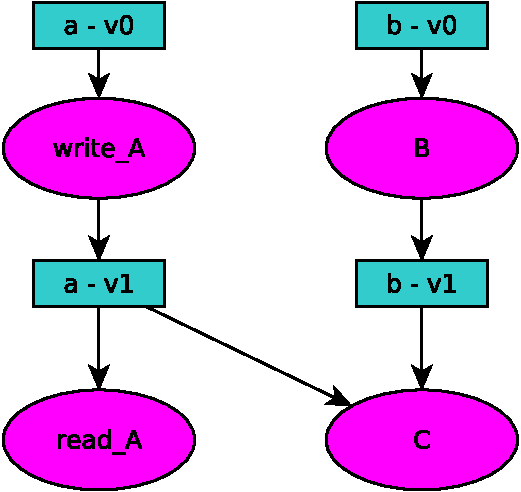
\includegraphics[width=0.5\textwidth]{dataflow-example}
  \caption{DAG équivalent au listing~\ref{lst:context:task-dep}}\label{fig:context:dag-dataflow}
\end{figure}

Exprimer son code avec des dépendances de données plutôt qu'avec des synchronisations globales permet de définir des synchronisations plus fines entre les différentes tâche, que le support exécutif peut utiliser pour minimiser le temps d'inactivité des ressources.
En effet, en utilisant des dépendances de données une tâche devient prête dès lors que ses données en lecture sont prêtes, ce qui, contrairement à une approche par synchronisation globale, est robuste à un déséquilibre de charge entre les tâches.


\subsection{Quelques exemples de modèles de programmation}\label{sec:context:others:examples}

Plusieurs modèles de programmation populaires proposent d'exprimer du parallélisme à base de tâches, parmi lesquels Cilk, OmpSs, et OpenMP, qui fonctionnent avec des approches légèrement différentes.
Le but de cette section est de comparer l'expression d'une même application, la factorisation de Cholesky, dans ces différents modèles.
Une comparaison plus large des supports exécutifs est effectuée dans la section~\ref{sec:rw:other-runtimes}.


\subsubsection{Code séquentiel de base}

La factorisation de Cholesky sera prise comme étude de cas et présentée en détails dans la section~\ref{sec:contribs:apps:cholesky}.
Le code séquentiel utilisé comme base pour la parallélisation est présenté dans le listing~\ref{lst:context:cholesky-seq}.

\begin{figure}[h!]
\begin{lstlisting}[language=c++,caption=Algorithme séquentiel,label=lst:context:cholesky-seq]
// Prototype des fonctions communes aux modèles de programmation
void dpotrf(double *A);
void dtrsm(double *A, double *B);
void dsyrk(double *A, double *B);
void dgemm(double *A, double *B, double *C);

// On suppose ici que l'expression A(i, j) retourne un pointeur
// vers le début du bloc i,j de la matrice A.
for (int k = 0; k < n_blocs; k++) {
  dpotrf(A(k, k));
  for (int m = k+1; m < n_blocs; m++)
    dtrsm(A(k, k), A(k, m));
  for (int m = k+1; m < n_blocs; m++) {
    for (int n = k+1; n < m; n++) {
      dgemm(A(k, n), A(k, m), A(n, m));
    }
    dsyrk(A(k, m), A(k, k));
  }
}
\end{lstlisting}
\end{figure}

\subsubsection{Cilk}

Cilk~\cite{cilk5} est un modèle de programmation basé sur C.
Il introduit principalement deux nouveaux mots clés : |spawn| et |sync|, pour, respectivement, exposer du parallélisme et introduire un point de synchronisation.
Le mot clé |spawn| vient précéder un appel de fonction pour indiquer que la fonction peut s'exécuter en parallèle. Cela en fait donc un modèle de programmation à base de tâches.
Cilk propose également une extension de la notation de tableau, ayant pour but de faciliter la vectorisation automatique par le compilateur.
La version parallélisée en Cilk est présentée dans le listing~\ref{lst:context:cilk}.


\begin{figure}[h!]
\begin{lstlisting}[language=c++,caption=Cholesky exprimé en Cilk,label=lst:context:cilk]
for (int k = 0; k < n_blocs; k++) {
  spawn dpotrf(A(k, k));
  sync;
  for (int m = k+1; m < n_blocs; m++)
    spawn dtrsm(A(k, k), A(k, m));
  sync;
  for (int m = k+1; m < n_blocs; m++) {
    for (int n = k+1; n < m; n++) {
      spawn dgemm(A(k, n), A(k, m), A(n, m));
    }
    spawn dsyrk(A(k, m), A(k, k));
    sync;
  }
}
\end{lstlisting}
\end{figure}


\subsubsection{OpenMP}

OpenMP~\cite{openmp45} est un modèle de programmation supportant le C/C++ et Fortran.
Le standard d'application de nos idées pour cette thèse étant OpenMP, une description détaillée des fonctionnalités et de ses spécificités est faite dans la section~\ref{sec:context:openmp}.

Contrairement à Cilk où la synchronisation est faite via un |sync| global, dans l'implémentation donnée dans le listing~\ref{lst:context:openmp} ce sont les dépendances de données qui induisent l'ordre d'exécution.

\begin{figure}[h!]
\begin{lstlisting}[language=c++,caption=Cholesky exprimé en OpenMP,label=lst:context:openmp]
for (int k = 0; k < n_blocs; k++) {
  #pragma omp task depend(inout:A(k,k))
  dpotrf(A(k, k));
  for (int m = k+1; m < n_blocs; m++) {
    #pragma omp task depend(in:A(k, k)) depend(inout:A(k, m))
    dtrsm(A(k, k), A(k, m));
  }
  for (int m = k+1; m < n_blocs; m++) {
    for (int n = k+1; n < m; n++) {
      #pragma omp task depend(in:A(k, n), A(k, m))
                       depend(inout:A(n, m))
      dgemm(A(k, n), A(k, m), A(n, m));
    }
    #pragma omp task depend(in:A(k, m)) depend(inout:A(k, k))
    dsyrk(A(k, m), A(k, k));
  }
}
\end{lstlisting}
\end{figure}

\subsubsection{OmpSs}

OmpSs~\cite{OMPSs} est un modèle de programmation proche d'OpenMP, mais où certaines \emph{déclarations} de fonctions sont marquées comme des tâches avec leurs dépendances (et leurs tailles associées).
Le listing~\ref{lst:context:cholesky-ompss} montre la factorisation de Cholesky exprimée en OmpSs.

\begin{figure}[h!]
\begin{lstlisting}[language=c++,caption=Cholesky exprimé en OmpSs,label=lst:context:cholesky-ompss]
// Taille de bloc
int bs = X;

#pragma omp task inout([bs][bs]A)
void dpotrf(double *A);
#pragma omp task in([bs][bs]A) inout([bs][bs]B)
void dtrsm(double *A, double *B);
#pragma omp task in([bs][bs]A) inout([bs][bs]B)
void dsyrk(double *A, double *B);
#pragma omp task in([bs][bs]A, [bs][bs]B) inout([bs][bs]C)
void dgemm(double *A, double *B, double *C);

for (int k = 0; k < n_blocs; k++) {
  dpotrf(A(k, k));

  for (int m = k+1; m < n_blocs; m++)
    dtrsm(A(k, k), A(k, m));

  for (int m = k+1; m < n_blocs; m++) {
    for (int n = k+1; n < m; n++) {
      dgemm(A(k, n), A(k, m), A(n, m));
    }
    dsyrk(A(k, m), A(k, k));
  }
}
\end{lstlisting}
\end{figure}


\subsubsection{Quelques autres modèles de programmation}

En plus des modèles présentés ci-dessus et des modèles abordés en détails dans la section~\ref{sec:rw:other-runtimes}, il existe un certain nombre de modèles de programmation à base de tâches, trop éloignés de nos travaux pour en faire une description approfondie.

Threading Building Block (TBB)~\cite{Reinders2007} est un modèle de programmation développé par Intel comme une bibliothèque C++.
Les tâches sont soumises au support exécutif via des fonctions mises à disposition du programmeur, qui doit passer en paramètre un pointeur vers une fonction au prototype prédéfini.

Hpx~\cite{Kaiser2014} est un modèle de programmation construit sur le modèle \emph{Partitioned Global Address Space}~\cite{PGAS}.
Il s'agit également d'une API C++, où les primitives de création de tâches prennent en paramètre un pointeur de fonction et une liste d'arguments à lui passer.

X10~\cite{Charles2005} est un langage basé sur Java et étendu implémenter un modèle PGAS.
Les opérations sur les tâches (création, synchronisation) se fait de manière similaire à Cilk, à l'aide de mots clés ajoutés dans le langage.
Il supporte une synchronisation fine des tâches à travers la notion de \emph{futures}~: le résultat d'une tâche peut être encapsulé dans un objet \emph{future}, sur lequel d'autres tâches peuvent se placer en attente.


\subsection{Quantité de travail et granularité}\label{sec:context:others:granularity}


Dans ce type de modèles de programmation, la clé pour maximiser l'utilisation des ressources est de réduire l'overhead du support exécutif par rapport au calcul en trouvant le bon \emph{grain} de tâche.

Il faut donc jouer sur le degré de parallélisme pour atteindre les meilleures performances : les tâches doivent être suffisamment petites pour proposer le maximum de parallélisme, mais pas trop pour ne pas surcharger le support exécutif, vis à vis des coûts décrits dans la section~\ref{sec:context:others:costs}.

Ce grain optimal dépend de plusieurs facteurs : les structures de données utilisées par le support exécutif, le coût de création des tâches, et la quantité de travail mis à disposition par cœur via ce grain.

Cela peut être illustré via une application telle que la factorisation de Cholesky par bloc présentée dans la section précédente : à taille de matrice fixée le nombre de tâches créées dépend directement de la taille de bloc choisie.
Plus la taille de bloc est petite, plus le nombre de blocs créés (et donc le nombre de tâches, et le parallélisme potentiel) est important.

\begin{figure}[ht]
  \centering
  \includegraphics[width=0.92\textwidth]{graph_granularity_8k_64.pdf}
  \caption{Performances de Cholesky pour une matrice de taille 8192 et 64 threads, en fonction de la taille de bloc}\label{fig:context:granularity}
\end{figure}

La figure~\ref{fig:context:granularity} illustre l'évolution des performances d'une factorisation de Cholesky d'une matrice de taille 8192, sur un nombre de cœurs fixé (64), en fonction de la taille de bloc et du support exécutif.
La machine utilisée pour cette expérience est \emph{idchire}, qui sera décrite en détails dans la section~\ref{sec:contribs:machines:idchire}.
De même une description détaillée des supports exécutif sera faite dans la section~\ref{sec:contribs:perf_eval:portage_libkomp} pour libKOMP, et dans la section~\ref{sec:rw:other-runtimes} pour les autres.

Comme on peut le voir, les parties extrèmes de la courbe se comportent de manière similaires quel que soit le support exécutif : une taille de bloc trop faible génère beaucoup trop de tâches et les support exécutifs sont complètement surchargés. Une taille de bloc trop importante limite complètement le parallélisme et donc les performances.

Le grain adapté n'est pas nécessairement unique : en fonction du support exécutif on peut avoir un choix plus ou moins important. Cela est illustré sur la figure~\ref{fig:context:granularity} : avec OmpSs le grain optimal se situe dans un intervalle de tailles de blocs assez restreint (entre environ 250 et 350), alors qu'avec clang ou libkomp une taille de bloc entre 150 et 350 permet d'obtenir des performances sensiblement équivalentes.

La courbe tracée avec libkomp inclut nos travaux sur l'affinité, et permet d'illustrer que même si l'affinité permet d'influer sur les performances maximales, elle n'a pas vraiment d'impact sur le grain optimal, comme cela est illustré sur la figure~\ref{fig:context:granularity-16k} (également réalisée sur la machine \emph{idchire}), ou le maximum de performance est obtenu pour tous les supports exécutifs aux environs de 300.

\begin{figure}[ht]
  \centering
  \includegraphics[width=0.92\textwidth]{graph_granularity_16k_64.pdf}
  \caption{Performances de Cholesky pour une matrice de taille 163384 et 64 threads, en fonction de la taille de bloc}\label{fig:context:granularity-16k}
\end{figure}


Le choix du grain pour une tâche dépend entièrement de l'application, et reste à l'appréciation du programmeur.

\bigskip

Bien que tous les modèles de programmation à base de tâches avec dépendances aient leur spécificités, ils permettent tous de décrire l'application sous forme de graphe de tâches direct et acyclique (DAG).

L'étape suivante consiste à exécuter ce graphe sur la machine, et pour cela le support exécutif peut se reposer sur un ensemble important de techniques d'ordonnancement. 


